% Adapted from TU Graz Template for ITI by Michael Krisper, Sept-2020
% Original Author: Maria Eichlseder
% Design based on the PowerPoint template by Christina Fraueneder
% Re-using some elements of the 2013 LaTeX template by Thomas Quaritsch
% both available at
% https://tu4u.tugraz.at/bedienstete/organisation-und-administration/vorlagen-und-corporate-design/downloads-und-anwendungen-logoformate-und-vorlagen/designlinien-und-vorlagen-download/charakteristika-designlinie-ic/vorlagen-download-designlinie-ic/
% See also https://latex.tugraz.at/vorlagen/tugraz and https://github.com/quam426/tugPoster

\documentclass{beamer} % 4:3 (default)
%\documentclass[aspectratio=169]{beamer}  % 16:9

\usetheme[institute,iti]{tugraz2018}

\usepackage[utf8]{inputenc}
\usepackage[english]{babel}

%% Add your own packages, macros, etc.
% ...

%% Enter presentation metadata
\title[Prediction with Regression on Universities Data Set]{Prediction with Regression\\on Universities Data Set\\\normalsize \\}
\author{\textbf{Group 14}: \\David Mihola, \\Ronald Infanger, \\Thomas Sterner}
\date{18. 06. 2023}

%% Logos
% \additionallogo{figures/logo}  % additional institute/department logo (footline; optional)
% \logobar{Supported by: ...}  % sponsors (titlepage; optional)


\begin{document}

\begin{frame}
  \maketitle
\end{frame}

\begin{frame}{Outline}
  \vspace{-1cm}
  \begin{enumerate}
      \item Data set analysis,
      \item cleaning and pre-processing,
      \item training and evaluation,
      \item regression models,
      \item prediction performance,
      \item ensemble.
  \end{enumerate}
\end{frame}


\begin{frame}{Data Set Analysis}
  TODO
\end{frame}
\begin{frame}{}
  \vspace{-0.3cm}
  \begin{figure}
    \centering
    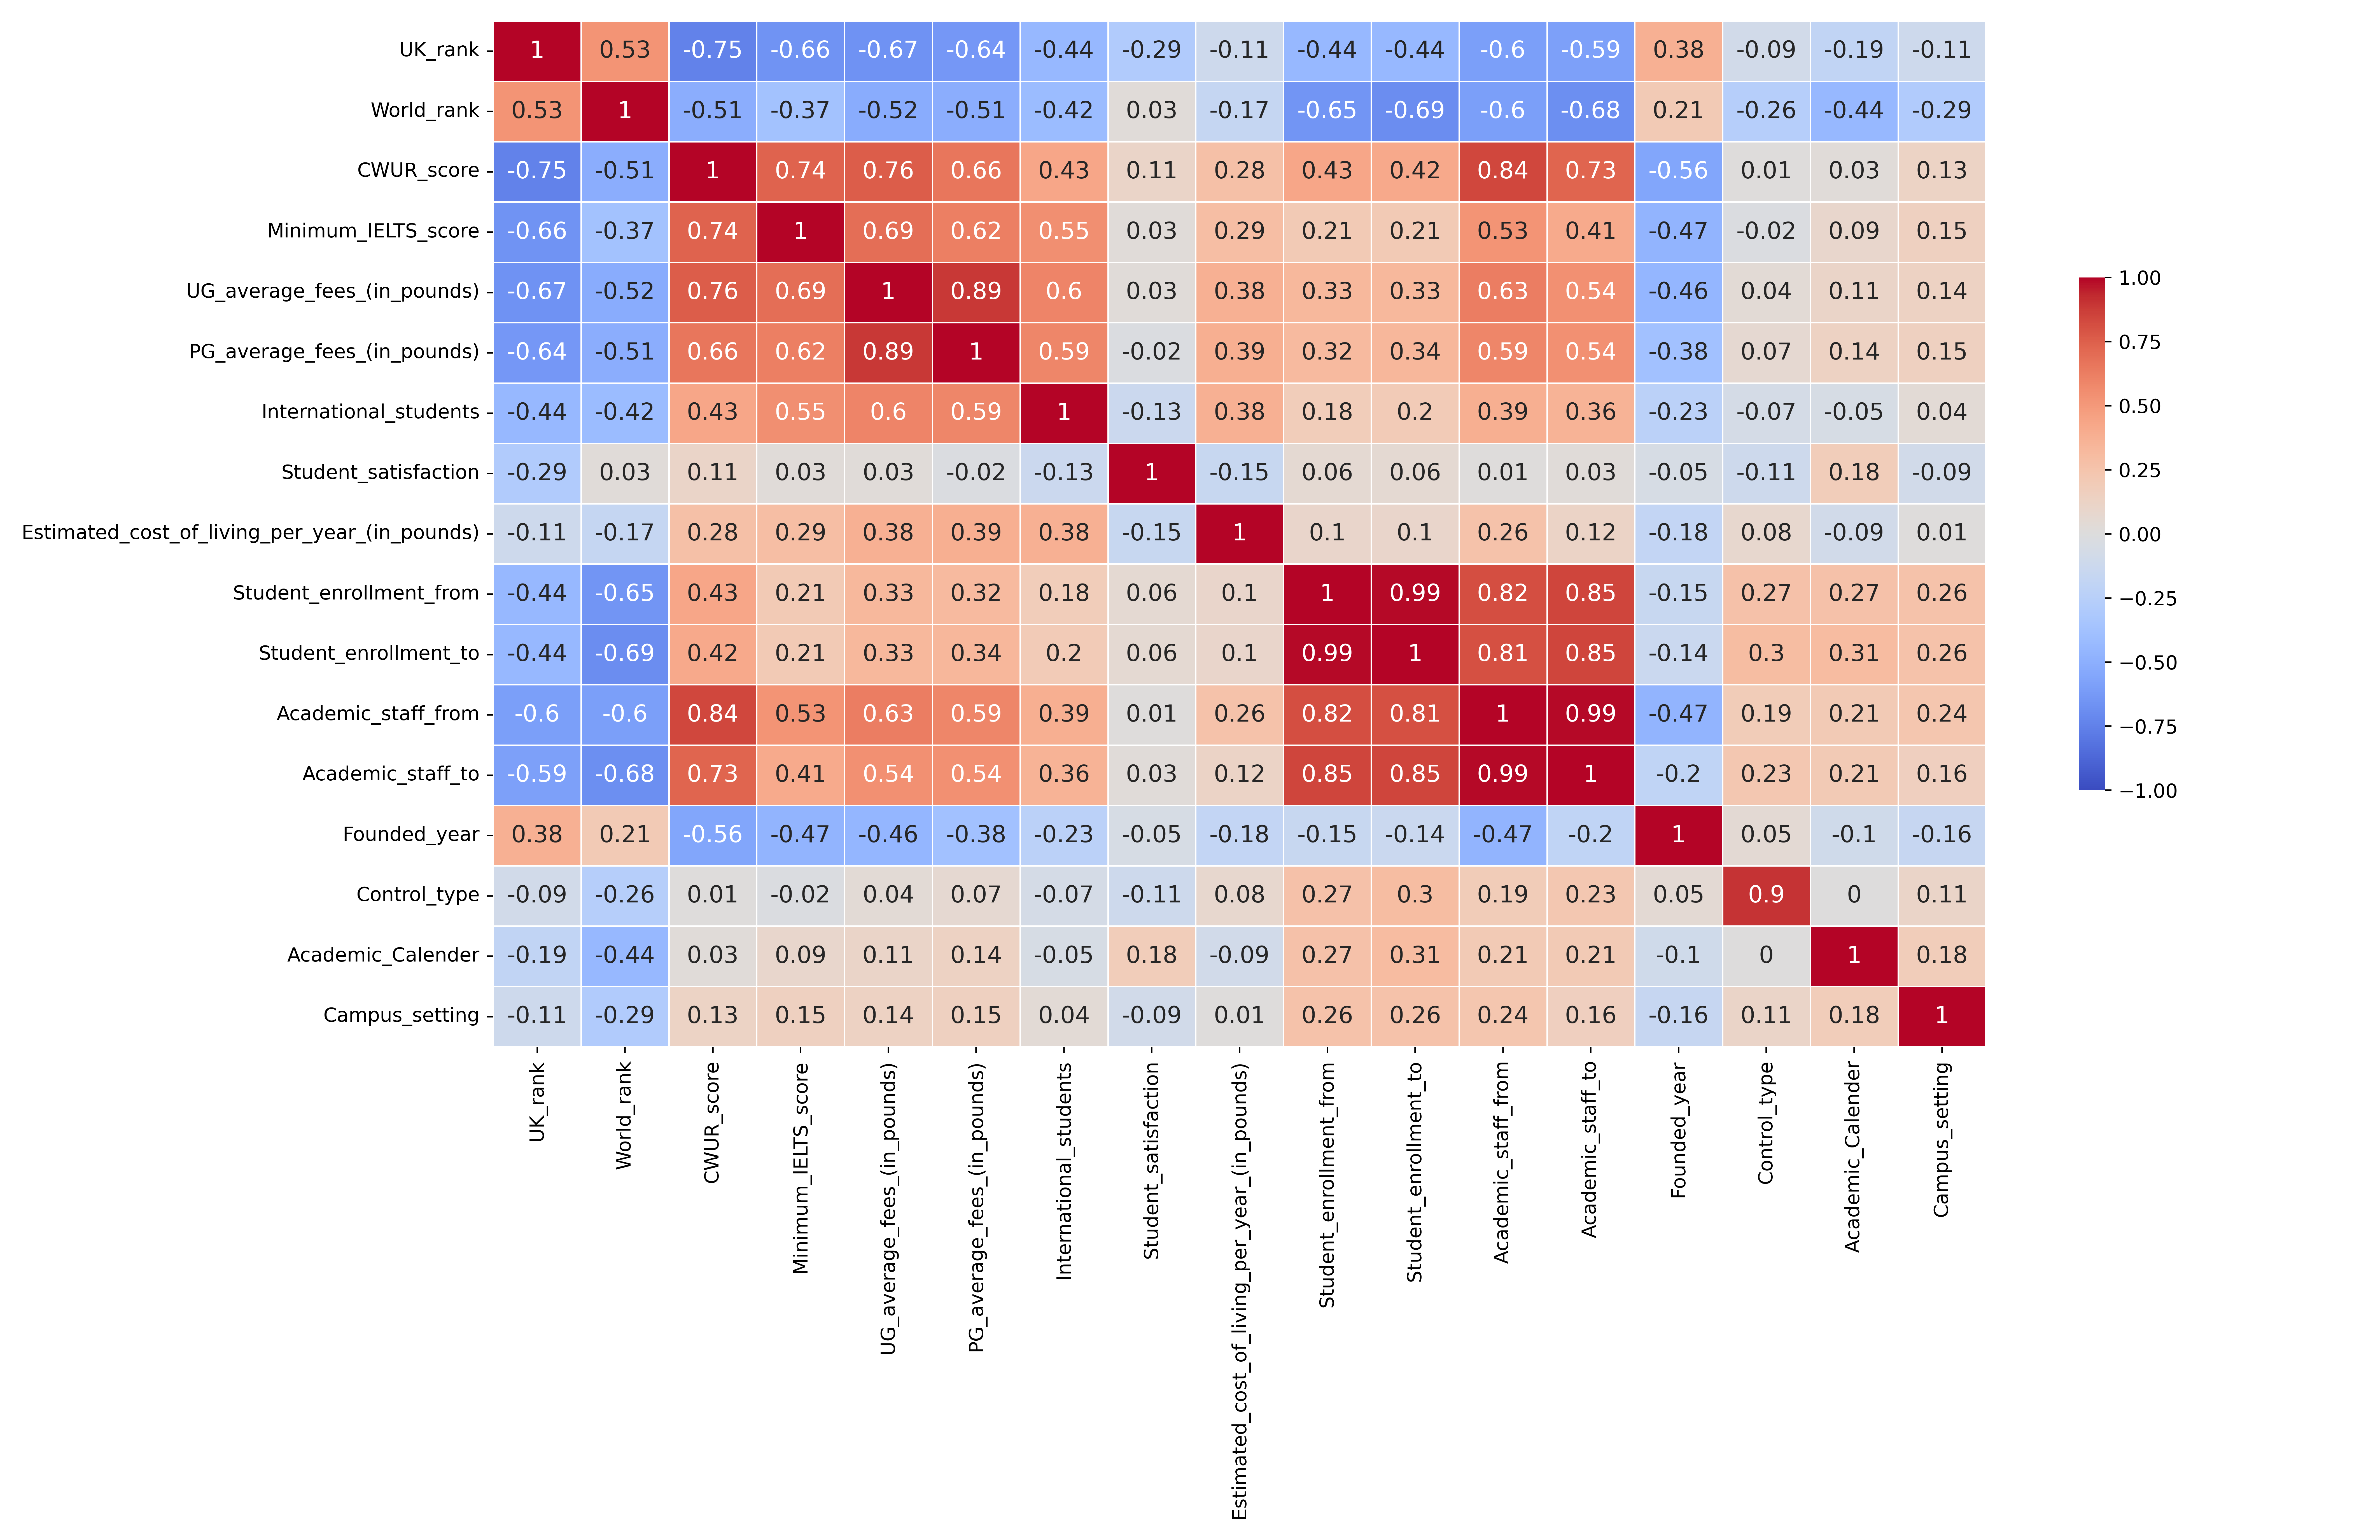
\includegraphics[width=0.94 \textwidth]{figs/correlation_heatmap.png}
    \caption{Correlation heat map}
    \label{fig:corr_heatmap}
\end{figure}
\end{frame}

\begin{frame}{Cleaning and Pre-processing}
  \vspace{-1cm}
  \begin{enumerate}
      \item Identification of missing values, split of compound columns, deduplication,
      \item data set split,
      \item missing value imputation,
      \item normalization,
      \item one-hot encoding,
      \item removal of non-numeric columns.
  \end{enumerate}
\end{frame}

\begin{frame}{Training and Evaluation}
  \vspace{-1cm}
  \begin{itemize}
      \item 3-fold cross validation (only on seed 14),
      \item 3 subsets of the data set:
        \begin{itemize}
            \item all continuous and categorical columns,
            \item only continuous columns excluding \texttt{Latitude} and \texttt{Longitude}
            \item columns with absolute value of correlation higher than 0.5 with the target variables
        \end{itemize}
      \item performance evaluation metrics: MSE, MAE, RMSE, R2 score,
      \item average performance across random seeds $[0, 4]$.
  \end{itemize}
\end{frame}

\begin{frame}{Models}
  \vspace{-0.5cm}
  Linear Regression
  \begin{itemize}
      \item baseline model to assess performance against,
      \item no cross validation.
  \end{itemize}
  Fully Connected Neural Network
  \begin{itemize}
      \item 3 architectures with:
        \begin{itemize}
            \item increasing number of hidden layers,
            \item ReLU hidden activation, linear output activation.
        \end{itemize}
  \end{itemize}
\end{frame}

\begin{frame}{Models}
  \vspace{-0.5cm}
  Random Forest
  \begin{itemize}
      \item grid search parameters:\\
      max features $[1, 10]$, N estimators $[1, 100]$.
  \end{itemize}
  Support Vector Regression
  \begin{itemize}
      \item grid search parameters:\\
      kernel (linear, poly, rbf, sigmoid), degree (2, 3, 4), epsilon [0, 0.2].
  \end{itemize}
\end{frame}

\begin{frame}{Prediction Performance and Ensemble}
  \begin{table}[ht!]
    \hspace{-0.9cm}
    \begin{tabular}{|c|c|c|c|c|}
        \hline
        & MSE & MAE & RMSE & R2 score\\
        \hline
        LR & 4127253.4 & 1362.20 & 1982.70 & 0.497 \\
        FCNN & 3024218.6 & 1167.42 & 1703.25 & 0.643 \\
        RF &  &  &  &  \\
        SVR &  &  &  &  \\
        \hline
    \end{tabular}
    \caption{Average prediction performance across random seeds $[0, 4]$ analyzed with different metrics}
    \label{tab:pred_perf}
\end{table}
\end{frame}

\end{document}
